% 4.11   2.14    lemma 6.8    lemma 6.9
\documentclass{article}
\DeclareMathAlphabet{\mathpzc}{OT1}{pzc}{m}{it}
\setlength{\parindent}{0pt}
\usepackage[table]{xcolor}
\usepackage{graphicx}
\usepackage{amssymb}
\usepackage{amsmath}
\usepackage{amsthm}
\usepackage{hyperref}
\usepackage{pgfplots}
\usepackage{pst-plot}
% \usepackage{fdsymbol}
\usepackage{empheq}
\usepackage{tikz}
\usepackage[most]{tcolorbox}
\usepackage{enumerate}
\usepackage{scalerel}
\usepackage{relsize}
\usepackage{mdframed}
\usepackage[utf8]{inputenc}

\usetikzlibrary{calc,patterns,angles,quotes}
\definecolor{myblue}{rgb}{2.55, 1.50, 0.20}
% \definecolor{myblue}{RGB}{227, 234, 253}
\newtcbtheorem[number within=subsection]{mytheo}{Sats}%
    {colback=myblue!15,colframe=black!30!black,
     enhanced,
     coltitle=black!75!black, boxrule=0.8pt,
     attach boxed title to top left=
       {xshift=2ex,yshift=-2mm,yshifttext=-1mm},
     boxed title style={colframe=black!30!black, boxrule=0.8pt,
       colback=myblue!60}}{th}

\newtcbtheorem[number within=subsection]{mydef}{Definition}%
    {colback=myblue!15,colframe=black!30!black,
     enhanced,
     coltitle=black!75!black, boxrule=0.8pt,
     attach boxed title to top left=
       {xshift=2ex,yshift=-2mm,yshifttext=-1mm},
     boxed title style={colframe=black!30!black, boxrule=0.8pt,
colback=myblue!60}}{th}

\newtcbtheorem[number within=subsection]{myprop}{Proposition}%
    {colback=myblue!15,colframe=black!30!black,
     enhanced,
     coltitle=black!75!black, boxrule=0.8pt,
     attach boxed title to top left=
       {xshift=2ex,yshift=-2mm,yshifttext=-1mm},
     boxed title style={colframe=black!30!black, boxrule=0.8pt,
colback=myblue!60}}{th}

\newtcbtheorem[number within=subsection]{mykol}{Korollarium}%
    {colback=myblue!15,colframe=black!30!black,
     enhanced,
     coltitle=black!75!black, boxrule=0.8pt,
     attach boxed title to top left=
       {xshift=2ex,yshift=-2mm,yshifttext=-1mm},
     boxed title style={colframe=black!30!black, boxrule=0.8pt,
colback=myblue!60}}{th}

\newtcbtheorem[number within=subsection]{mylemma}{Lemma}%
    {colback=myblue!15,colframe=black!30!black,
     enhanced,
     coltitle=black!75!black, boxrule=0.8pt,
     attach boxed title to top left=
       {xshift=2ex,yshift=-2mm,yshifttext=-1mm},
     boxed title style={colframe=black!30!black, boxrule=0.8pt,
colback=myblue!60}}{th}

% ---------------------------------------------
% ---------------RE-NEW COMMAND----------------
% ---------------------------------------------
\newcommand\mul[1]{\multicolumn{1}{c}{#1}}
\setlength{\parskip}{1em}
\renewcommand{\baselinestretch}{1.2}
\renewcommand*{\proofname}{Bevis}
\newcommand{\ovning}[1]{\noindent {\bf Övning #1.}}
\renewcommand{\contentsname}{Innehåll}
\newcommand{\orbit}[0]{\mathlarger{\mathlarger{\mathcal{O}}}}
\newcommand{\grad}[0]{\textnormal{deg}}
\newtheorem{definition}{Definition}[section]
\pgfplotsset{compat=1.8}

\theoremstyle{definition}
\newtheorem{thm}{Theorem}[section]
\newtheorem{exmp}[thm]{Exempel}
\begin{document}
\title{%
  Galoisteori och de olösbara polynomen \\
  \small{En introduktion till det abstrakta - Del II}
}
\author{Gabriel Rajkowski}
\date{\today}

\maketitle

\thispagestyle{empty}

\clearpage
\tableofcontents
\section{Inledning}
\section{Historia}
\section{Komplement till del I}
Denna del ägnar sig åt saker som inte togs upp i del I på grund av de inte fick plats eller som inte var nödvändiga men som kommer att komma 
till hands i denna del.

\subsection{Linjär algebra}
En stor sak som undveks i del I var vektorrum. Det visar sig faktiskt att vektorrum blir väldigt praktiska och går hand i hand med andra 
algebraiska strukturer såsom kroppar och dess utvidgningar. I detta delavsnitt kommer vi att studera grunderna för vektorrum så att de senare kan användas till 
våran fördel.

\begin{mydef}{Vektorrum}{}
  Ett vektorrum över en kropp (vi definerar detta senare) $F$ är en mängd $V$ under addition och subtraktion som uppfyller följande axiom.
  \begin{enumerate}[I)]
    \item $V$ skapar en abelsk grupp under addition,
    \item $a \cdot (b \cdot v) = (a \cdot b) \cdot v$,
    \item $1 \cdot v = v$ där 1 är den multiplikativa enhetselementet i $F$,
    \item $a \cdot (u + v) = (a \cdot u) + (a \cdot v)$,
    \item $(a + b) \cdot v = (a \cdot v) + (b \cdot v$),
  \end{enumerate}
  där $a, b \in F$ och $v, u \in V$.
\end{mydef}
Elementen i $F$ brukar kallas för skalärer och elementen i $v$ 
brukar kallas för vektorer. 

% \begin{mydef}{Linjära beroenden}{}
%   Låt $v_1, v_2, \cdots, v_n$ vara element i ett vektorrum 
%   $V$ över en kropp $F$ och låt $a_1, a_2, \cdots, a_n \in F$.
%   Vektorerna är \textit{linjärt oberoende} om ekvationen 
%   \[a_1v_1 + a_2v_2 + \cdot + a_nv_n = 0\]
%   endast har lösningen $a_1 = a_2 = \ldots a_n = 0$.
%   Om sådant inte är fallet, det vill säga då 
%   en vektor kan skrivas som en linjär kombination av de andra, 
%   så är vektorerna \textit{linjärt beroende}.
% \end{mydef}
(några exempel)

\begin{mydef}{Baser}{}
  En delmängd $K$ av ett vektorrum $V$ över en kropp $F$ är en \textit{bas} för $V$ om följande villkor uppfylls.  
  \begin{enumerate}[I)]
    \item $K$ är \textit{linjärt oberoende}. För $v_1, \ldots, v_n \in K$ och $a_1, \ldots, a_n \in F$ så har ekvationen 
    \[a_1v_1 + \cdots + a_n v_n = 0\]
    lösningen $a_1 = \cdots = a_n = 0$.
    \item $K$ \textit{spänner upp} $V$. För alla $v \in V$ så existerar det $b_1, \ldots b_m \in F$ och $v_1, \ldots v_m \in K$ så att 
    $v = b_1 v_1 + \cdots + b_m v_m$.
  \end{enumerate}
\end{mydef}

\subsection{Gruppteori}
Detta avsnitt kommer ägna sig åt normala delgrupper och kvotgrupper. Dessa blir mycket nödvändiga för oss när vi ska bevisa textens viktigaste sats. 
Mer specifikt kommer vi vara intresserade av kedjor av normala delgrupper och om deras kvotgrupp är abelsk eller icke. Denna 
del kommer även underlätta senare koncept inom ringteori.

\begin{mydef}{Normala delgrupper}{}
  Låt $N$ vara en delgrupp till $G$. Vi säger att $N$ är 
  en \textit{normal delgrupp} till $G$ om $N$ är 
  \textit{invariant under kojugering}, för alla $n \in N$ och 
  alla $g \in G$ så är $gng^{-1} \in N$. Vi skriver då $N \triangleleft G.$
\end{mydef}
Motivationen bakom denna till synes konstiga definition finner man i kvotgrupper. 
En definerande egenskap hos normala delgrupper tas upp i följande proposition.

\hypertarget{prop1}{}
\begin{myprop}{}{}
  Låt $N$ vara en normal delgrupp till $G$ och $g \in G$. Vänstersidoklassen till $N$ är då lika med högersidoklassen till $N$ med avseende på $g$, 
  $gN = Ng.$
\end{myprop}
\begin{proof}
  Om $n \in N$ så är $gn \in gN$. Notera nu att 
  \begin{equation*}
    gn = gn(g^{-1}g) = \underbrace{(gng^{-1})}_{ \substack{N \triangleleft G  \implies \\ gng^{-1} \in N}} g.
  \end{equation*}
  Detta visar att $gN \subseteq Ng.$ Ett godtyckligt element i $Ng$ är på formen $ng$. Observera att 
  \begin{equation*}
    ng = n(g^{-1})^{-1} = g \underbrace{g^{-1} {n(g^{-1})^{-1}}}_{\substack{N \triangleleft G  \implies \\ g^{-1} {n(g^{-1})^{-1} \in N}}}.
  \end{equation*}
  Detta visar att $Ng \subseteq gN$ vilket slutför beviset.
\end{proof}

\begin{mydef}{Kvotgrupper}{}
  Låt $N$ vara en normal delgrupp till $G$. \textit{Kvotgruppen} $G/N$, som utläses "$G$ modulo (mod) $N$", är gruppen innehållande alla 
  sidoklasser till $N$, 
  \[G/N \equiv \{gN \; | \; g \in G\},\]
  där gruppoperationen defineras som $(aN) (bN) = (ab)N$. 
\end{mydef}
Denna definition använder sig av vänstersidoklasser men, enligt \hyperlink{prop1}{proposition 3.2.1}, så kan man lika gärna använda sig 
av högersidoklasser. Notera att för $a' \in aN, a \in G$ så är $a'N = aN$ enligt resultat från del I. Det vi har kvar att visa är att $(a'N) (b'N) = (ab)N
\iff (a'b')N = (ab)N$, det vill säga att det inte spelar någon roll vilka representanter framför $N$, $a' \in aN, b' \in bN$, vi väljer. Resultatet av 
operationen bör vara oberoende av vilka representanter vi väljer, annars skulle det kunna finnas flera svar till en och samma sak. Med 
andra ord måste vi visa att operationen är \textit{väldefinerad}.

För att visa detta kan vi låta $a' \in aN$ och $b' \in bN$. Vi kan skriva dessa som $a' = an_1$ och $b' = bn_2$ för $n_1, n_2 \in N$. Med denna 
omskrivning kan vi konstatera att
\[(a'b')N = (an_1bn_2)N.\]
Eftersom assosiativitet gäller så är 
\[(an_1bn_2)N = an_1b(n_2N).\]
Vidare har vi även att $n_2 \in N$ vilket enligt resultat från del I ger 
\[an_1b(n_2N) = an_1bN.\]
Enligt \hyperlink{prop1}{proposition 3.2.1} har vi att 
\[an_1bN = ab(n_1N) = (ab)N.\]

Vi vet från del I att mängden av sidklasser utgör en partition av en grupp och därför är följande figur lämplig.

\begin{center}
  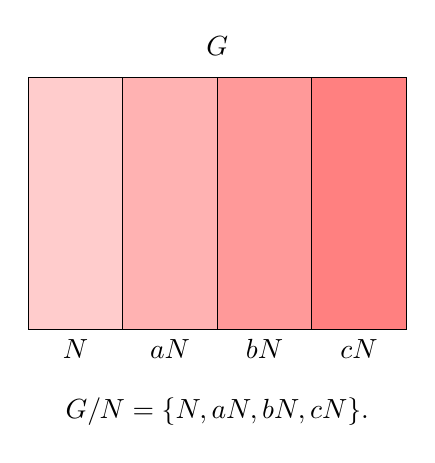
\begin{tikzpicture}[scale=0.8]
    \node at (0, 2.5) {$G$};
    \draw (-3,2) rectangle (3,-2);
    \foreach \i [count=\xi] in {-3, -1.5,..., 0}{
      \draw (\i, 2) rectangle (-\i, -2);
    }
    \node at (-2.25, -2.3) {$N$};
    \node at (-0.75, -2.3) {$aN$};
    \node at (0.75, -2.3) {$bN$};
    \node at (2.25, -2.3) {$cN$};
    \node at (0, -3.3) {$G/N = \{N, aN, bN, cN\}.$};

    \draw[fill = red!20] (-3, 2) rectangle (-1.5, -2);
    \draw[fill = red!30] (-1.5, 2) rectangle (0, -2);
    \draw[fill = red!40] (0, 2) rectangle (1.5, -2);
    \draw[fill = red!50] (1.5, 2) rectangle (3, -2);
  \end{tikzpicture}
\end{center}
Man kan alltså tänka sig att en kvotgrupp $G/N$ delar upp $G$ i mindre delar vars storlek är $|N|$. 

\begin{exmp}
  Vi vet att $\mathbb{Z}$ är en grupp under addition och att $3 \mathbb{Z}$ är en normal delgrupp till $\mathbb{Z}$, ty $z + n + (-z) \in 3 \mathbb{Z}$
  för $z \in \mathbb{Z}, n \in 3 \mathbb{Z}$. Alla möjliga sidoklasser till $3 \mathbb{Z}$ är $3 \mathbb{Z} + 1$ och $3 \mathbb{Z} + 2$ och därför är 
  $\mathbb{Z} / 3\mathbb{Z} = \{3 \mathbb{Z}, \; 3 \mathbb{Z} + 1, \; 3 \mathbb{Z} + 2\}$. Man brukar beteckna $3 \mathbb{Z}$ med $[0]$, 
  $3 \mathbb{Z} + 1$ med $[1]$ och $3 \mathbb{Z} + 2$ med $[2]$. Med dessa beteckningar blir $\mathbb{Z} / 3\mathbb{Z} = \{[0], [1], [2]\}$. 
  Med hjälp av figuren 
  nedan, som visar Cayleytabellen för denna grupp respektive den cykliska gruppen av ordning tre, så kan vi konstatera att
  \[\mathbb{Z} / 3\mathbb{Z} \cong C_3 \cong (\mathbb{Z}_3, +).\]
  \begin{center}
    \begin{tabular}{c | c c c}
      $+$ & $[0]$ & $[1]$ & $[2]$  \\
      \cline{1-4}
      $[0]$ & $[0]$ & $[1]$ & $[2]$ \\
      $[1]$ & $[1]$  & $[2]$ & $[e]$\\
      $[2]$ & $[2]$ & $[e]$  & $[1]$\\
    \end{tabular} 
    \qquad
    \begin{tabular}{c | c c c}
      $\circ$ & $e$ & $\sigma$ & $\sigma^2$ \\
      \cline{1-4}
      $e$ & $e$ & $\sigma$ & $\sigma^2$ \\
      $\sigma$ & $\sigma$ & $\sigma^2$  & $e$\\
      $\sigma^2$ & $\sigma^2$ & $e$ & $\sigma$
    \end{tabular}
  \end{center}
  Till exempel så är $[2] + [1] = (3 \mathbb{Z} + 2) + (3 \mathbb{Z} + 1) = 3\mathbb{Z} + 3 = 3 \mathbb{Z} = [0].$
\end{exmp}
Man kan enkelt visa att en kvotgrupp faktiskt bildar en grupp och därför lämnas detta som en övning till läsaren.
\section{Ringar, kroppar och polynom}
\subsection{Ringar}
Precis som vektorrum så går det att använda ringar till våran fördel genom hela texten, speciellt då vi kommer till
Galoisteorins fundamentalsats.
\begin{mydef}{Ringar}{}
  En \textit{ring} är en mängd med två operationer plus, $+$, och multiplikation $\cdot$, som uppfyller följande \textit{ringaxiom}.
  \begin{enumerate}[I)]
    \item Ringen $R$ bildar en abelsk grupp under addition,
    \item ringen $R$ bildar en \textit{monoid} under multiplikation, det vill säga 
    \begin{enumerate}
      \item $(a \cdot b) \cdot c = a \cdot (b \cdot c)$,
      \item det finns ett \textit{multiplikativt enhetselement} $1 \in R$ så att $1 \cdot a = a \cdot 1,$
    \end{enumerate}
    \item multiplikation är distributiv över addition, $a \cdot (b+c) = (a \cdot b) + (a \cdot c)$ och $(b + c) \cdot a = (b \cdot a) + (c \cdot a),$
  \end{enumerate}
  för alla $a, b, c \in R$. Om multiplikation är kommutativ över $R$ så säger vi att $R$ är en \textit{kommutativ ring}. 
\end{mydef}
Ibland definieras en ring utan axiom II b) men i denna text finns denna med och därför, om inte något annat nämns, så antas en ring ha ett multiplikativt enhetselement. 
En ring utan detta axiom brukar kallas för en rng som uttalas \textit{rung}. Eftersom vi endast är intresserade av kommutativa ringar så kommer vi 
att benämna varje kommutativ ring för en ring. 

\begin{mydef}{Ideal}{}
  Låt $R$ vara en ring och $I$ vara en delmängd till denna. Vi säger att $I$ är ett \textit{ideal} om $I$ är en additativ delgrupp till $R$
  och om $i \in I$ samt $r \in R$ så är $i \cdot r \in I$. 
\end{mydef}
Det följer från definitionen att $ab \in I$ för alla $a, b \in I$ och $I$ är därför sluten under multiplikation. Detta faktum tillsammans 
med att ett ideal är sluten under addition och att ett ideal är en delmängd betyder att det är en \textit{delring}.
Notera även att ett ideal egentligen är en rng då $1 \notin I$. Om detta var fallet skulle 
$r = 1r \in I$ för alla $R$ och $I$ skulle därför inte vara en delmängd till $R$. 

Anledningen till varför det är intressant att studera ideal är av precis samma anledning till varför det är intressant att studera normala delgrupper, 
vi kan nämligen skapa kvotringar med hjälp av ideal.

\begin{mydef}{Kvotringar}{}
  Låt $I$ vara ett ideal till $R$. \textit{Kvotringen} $R/I$, som utläses "$R$ modulo (mod) $I$, är ringen innehållande alla sidoklasser till $I$, 
  \[R/I \equiv \{I + r \; | \; r \in R\}.\]
\end{mydef}

Vi vet från att ha studerat kvotgrupper att kvotgruppen $(R/I, +)$ skapar en grupp med operationen 
\[ (I + r_1) + (I + r_2) = I + (r_1 + r_2).\]
Vi har även observerat att denna operation är väldefinerad om en normal delgrupp väljs. I detta fall jobbar vi med ringar, det vill säga 
$(R, +)$ är abelsk, och därför är även operationen väldefinerad med ideal. Notera att $(R/I, +)$ är abelsk eftersom $(R, +)$ är abelsk.

Vi kan definera multiplikation av elementen i kvotringen $R/I$ på ett liknande sätt:
\[(I + r_1) \cdot (I + r_2) = I + (r_1 \cdot r_2). \]
För att visa att detta är väldefinerat så låter vi $r_1' \in I + r_1$ och $r_2' \in I + r_2$ för $r_1, r_2 \in R$. Vi kan skriva 
om $r_1'$ som $r_1' = i_1 + r_1$ och $r_2'$ som $r_2' = i_2 + r_2$ för $i_1, i_2 \in I$. Med denna omskrivning kan vi observera följande.
\[(I + r_1') \cdot (I + r_2') = (I + (i_1 + r_1)) \cdot (I + (i_2 + r_2))\]
och per definition får vi 
\[(I + (i_1 + r_1)) \cdot (I + (i_2 + r_2)) = I + ((i_1 + r_1) \cdot (i_2 + r_2)).\]
Eftersom multiplikation är distributiv över addition fås (i följande rad har $\cdot$ utelämnats)
\[I + ((i_1 + r_1) \cdot (i_2 + r_2)) = I + (\underbrace{i_1  i_2 + i_1  r_2 + r_1  i_2}_{\in I} + r_1  r_2).\]
Den delen som är understrycken tillhör $I$ eftersom det är ett ideal. Vi kallar denna del för $i_3$. Detta ger
\[I + (i_3 + r_1 \cdot r_2) = (I + i_3) + (I + r_1 \cdot r_2).\]
Tidigare resultat från del I ger 
\[(I + i_3) + (I + (r_1 \cdot r_2)) = I + (r_1 \cdot r_2)\]
och operationen är således väldefinerad. 

VISA ATT DETTA ÄR EN RING... !!!

\begin{mydef}{Ring homomorfism och isomorfism}{}
  Låt $R$ och $S$ vara ringar. En \textit{ring homomorfism} $\varphi: R \rightarrow S$ är en funktion så att 
  \begin{enumerate}[I)]
    \item $\varphi(r_1 + r_2) = \varphi(r_1) + \varphi(r_2)$,
    \item $\varphi(r_1 \cdot r_2) = \varphi(r_1) \cdot \varphi(r_2)$
  \end{enumerate}
  för alla $r_1, r_2 \in R$. En bijektiv ring homomorfism kallas för en \textit{ring isomorfism}.
\end{mydef}
En ring homomorfism är alltså en grupp homomorfism men för "både addition och multiplikation".

\begin{mydef}{Kärnan och bilden av en homomorfism}{}
  Låt $R$ och $S$ vara ringar och $\varphi: R \rightarrow S$ en homomorfism. \textit{Kärnan} av $\varphi$
  defineras som 
  \[ker(\varphi) \equiv \{r \in R \; | \; \varphi(r) = 0\}.\]
  \textit{Bilden} av $\varphi$ defineras som 
  \[Im(\varphi) \equiv \{\varphi(r) \; | \; r \in R\}.\]
\end{mydef}
Detta togs även upp i del I.
\begin{mytheo}{First isomorphism theorem}{}
a  
\end{mytheo}

\subsection{Kroppar}
För att börja med Galoisteori så måste vi först ha en plats där vi kan utföra vanlig aritmetik, en \textit{kropp}. Galoisteori kan ses som en studie 
av dessa platser som tillåter grundläggande aritmetik och dess relation till polynom. Vi skall i detta delavsnitt och i avsnittet "kroppsutvidgningar" 
presentera de huvudsakliga faktan om 
sådana strukturer. 


\begin{mydef}{Kroppar}{}
    En \textit{kropp} är en mängd $F$ under två binära operationer, addition ($+$) och multiplikation ($\cdot$), som uppfyller följande \textit{kroppsaxiom}.
    \begin{enumerate}[I)]
        \item \textbf{Assosiativitet.} $a + (b + c) = (a + b) + c$ och $a \cdot (b \cdot c) = (a \cdot b) \cdot c$.
        \item \textbf{Kommutativitet.} $a + b = b + a$ och $a \cdot b = b \cdot a$.
        \item \textbf{Additativa och multiplikativa enhetselementet.} Det existerar två olika element $0$ och $1$ så att $a + 0 = a$ och $a \cdot 1 = a.$
        \item \textbf{Additativ invers.} För alla $a$ så existerar det en \textit{additativ invers} till $a$, som betecknas
        $-a$, så att $a + (-a) = 0$.
        \item \textbf{Multiplikativ invers.} För alla $a \neq 0$ så existerar det en \textit{multiplikativ invers} till $a$, som betecknas $a^{-1}$ eller $1/a$, så att 
        $a \cdot a^{-1} = 1.$
        \item \textbf{Distributivitet av multiplikation över addition.} $a \cdot (b + c) = (a \cdot b) + (a \cdot c)$,
    \end{enumerate}
    för $a, b, c \in F$
\end{mydef}
En kropp skapar alltså en abelsk grupp under addition och kroppen utom $0$ skapar en abelsk grupp under multiplikation. Alternativt kan en kropp sägas
vara en kommutativ ring. Om $K$ är en kroppsutvidgning till $F$ så kommer vi säga att $F$ är baskroppen. 


\begin{mydef}{Karakteristik}{}
  Låt $F$ vara en kropp. Om det existerar ett minsta positiva tal $n$ så att $\underbrace{1 + \cdots + 1}_{n} = 0$ så kallas $n$ för kroppens \textit{karakteristik}.
  Om $n$ inte existerar är karakteristiken för kroppen $0.$
\end{mydef}
Man kan göra en koppling mellan karakteristik och cykliska grupper där alla element genereras genom ett enda element. Om en kropps karakteristik inte är noll
så kan den anses vara "cyklisk". 

\subsection{Polynom}
\begin{mydef}{Polynom}{}
  Låt $F$ vara en kropp. Ett \textit{polynom} över $F$ är en ekvation på följande form
  \[f(X) = a_0 + a_1X + a_2X^2 + \cdots a_nX^n\]
  där $n \in \mathbb{N}$ och där \textit{koefficienterna} $a_1, a_2, \ldots, a_n \in F$. 
  Mängden $F[X]$ består av alla polynom vars koeffcienter tillhör $F$. \textit{Graden} för ett polynom är den högsta multipliciteten av den obestämda variablen som förekommer i  
  polynomet och betecknas $\grad f(X)$. (För polynomet ovan är $\grad f(X) = n$.)
\end{mydef}
Trots att $\mathbb{Z}$ inte är en kropp så kommer vi fortfarande beteckna $\mathbb{Z}[X]$ som mängden av polynom med heltals koeffcienter
för att slippa skriva mycket.

\begin{mydef}{Irreducibla polynom}{}
  Låt $f(X)$ vara ett polynom över kroppen $F$. Vi säger att $f(X)$ är \textit{irreducibelt} över $F$ om det inte kan faktoriseras som $f(X) = g(X)h(X)$
  för $g(X), h(X) \in F[X]$ vars grad är mindre än $f(X)$. Om faktoriseringen går att åstadkomma säger vi att $f(X)$ är \textit{reducibelt} över $F.$
\end{mydef}
Notera att denna faktorisering beror starkt på vilken kropp en jobbar med. I till exempel $\mathbb{Q}[X]$ finns det endast några "få" polynom som är reducibla
över $\mathbb{Q}[X]$, medan alla polynom över $\mathbb{C}[X]$ är reducibla över $\mathbb{C}[X]$. Det sistnämnda är algebrans fundemental sats och 
bevisas senare i texten.

Nedan följer några exempel på metoder för att visa att polynom är irreducibla. 
(några övningar eller exempel, beroende på vad jag väljer)

\begin{mylemma}{Gauss's lemma}{}
Låt $f(X)$ vara ett polynom med heltals koeffcienter. Då är $f(X)$ irreducibel över $\mathbb{Z}$ om och endast om den är irreducibel över $\mathbb{Q}$.
\end{mylemma}
\begin{proof}
  Det som skall bevisas är följande
  \begin{align*}
    f(X) \textnormal{ är irreducibel över } \mathbb{Z} &\Rightarrow f(X) \textnormal{ är irreducibel över } \mathbb{Q}, \\
    f(X) \textnormal{ är irreducibel över } \mathbb{Q} &\Rightarrow f(X) \textnormal{ är irreducibel över } \mathbb{Z}.
  \end{align*}
  Påståendet är ekvivalent med det kontrapositiva påståendet.
  \begin{align}
    f(X) \textnormal{ är reducibel över } \mathbb{Q} &\Rightarrow f(X) \textnormal{ är reducibel över } \mathbb{Z}, \\
    f(X) \textnormal{ är reducibel över } \mathbb{Z} &\Rightarrow f(X) \textnormal{ är reducibel över } \mathbb{Q}.
  \end{align}
  Påstående (2) är trivial, då $\mathbb{Z}[X]$ är en delmängd till $\mathbb{Q}[X]$ (ett heltal är även ett rationellt tal). Vi bevisar påstående (2),
  att om $f(X)$ är reducibel över $\mathbb{Q}$ så medför detta att den också är reducibel över $\mathbb{Z}$. Anta att
  \begin{equation}
    f(X) = g_1(X)g_2(X)
  \end{equation}
  där $g_1(X), \; g_2(X) \in \mathbb{Q}[X]$. Eftersom koefficienterna för $g_1(X)$ och $g_2(X)$ är rationella tal så kan vi multiplicera med ett
  heltal $n$ i båda led i (3) som delar alla koefficienternas nämnare hos $g_1(X)$ och $g_2(X)$. Vi får då ekvationen
  \begin{equation}
    nf(X) = h_1(X)h_2(X)
  \end{equation}
  där $h_1(X), \; h_2(X) \in \mathbb{Z}[X]$. Bland alla dessa uttryck, välj $n$ till det minsta positiva heltalet
  så att faktoriseringen går att utföra. Vi påstår att $n = 1$ som då kommer att slutföra beviset. Vi antar motsatsen, att $n$ inte är 1. Eftersom 
  $n$ delar alla nämnare hos $g_1(X)$ och $g_2(X)$ så kan det inte vara ett primtal och därför måste ett primtal dela $n$. Kalla detta primtal för $p$, då 
  måste även $p$ dela högerledet, $h_1(X)h_2(X)$, eftersom $p$ delar vänsterledet. Anta att 
  \[h_1(X) = a_0 + a_1X + \cdots + a_lX^l, \quad h_2(X) = b_0 + b_1X + \cdots + b_mX^m\]
  för Vi påstår att $p$ antigen delar alla $a_i$ eller alla $b_i$. Antag motsatsen. Det finns nu två olika motsatser som kan antas.
  \begin{enumerate}[I)]
    \item Antigen delar $p$ några $a_i$ \textit{eller} några $b_i$,
    \item $p$ delar några $a_i$ \textit{och} några $b_i$.
  \end{enumerate}
  Påstående I) är falsk då alla koeffcienter i $h_1(X)h_2(X)$ måste vara delbara med $p$ och om endast några koeffcienter i det ena polynomet 
  är delbara med $p$ men inte i den andra så uppfylls detta inte. 

  Vi antar att påstående II) gäller. Det är då lämpligt att anta att $p$ delar $a_0, a_{1}, \ldots, a_{j-1}$ men inte $a_j$ och att 
  $p$ delar $b_0, b_{1}, \ldots, b_{k-1}$ men inte $b_k$. Observera att
  \[c_{j+k} = a_0b_{j+k} + \cdots + a_{j-1}b_{k+1} + a_jb_k + a_{j+1}b_{k-1} + \cdots + a_{j+k}b_0\]
  är en koeffcient i $f(X)$ och $p$ måste därför dela $c_{j+k}$. Vi vet även att $p$ delar $a_0, a_{1}, \ldots, a_{j-1}, b_0, b_{1}, \ldots, b_{k-1}$ 
  och därför måste $p$ dela $a_j b_k$. Detta leder till en motsägelse eftersom $p$ måste isåfall dela $a_j$ och/eller $b_k$ och vi drar slutsatsen att 
  $p$ delar alla koeffcienter i $h_1(X)$ eller alla koeffcienter i $h_2(X)$. Låt oss anta det förra. Definera nu 
  \[h_1'(X) = \frac{1}{p} h_1(X)\]
  som, enligt det ovanstående antagandet, tillhör $\mathbb{Z}[X].$ Vi kan därför dela (4) med $p$ för att få
  \[\frac{n}{p} f(X) = h_1'(X) h_2(X).\]
  Detta strider mot antagandet att $n$ är minimal och vi kan konstatera att $n=1$. Detta slutför beviset för lemmat.
\end{proof}

\begin{mytheo}{Eisensteins kriterium}{}
  Låt
  \[f(X) = a_0 + a_1X + \cdots + a_nX^n\]
  vara ett polynom över $\mathbb{Z}$. Om det existerar ett primtal $p$ så att 
  \begin{enumerate}[I)]
    \item $p$ inte delar $a_n$,
    \item $p$ delar $a_0, a_1, \ldots, a_{n-1}$,
    \item $p^2$ inte delar $a_0$,
  \end{enumerate}
  så är $f(X)$ irreducibel över $\mathbb{Q}$.
\end{mytheo}
\begin{proof}
  Enligt Gauss's lemma räcker det med att visa att $f(X)$ är irreducibel över $\mathbb{Z}$. Anta att $f(X) = g_1(X) g_2(X)$ där 
  \[g_1(X) = b_0 + b_1X + \cdots b_kX^k, \quad g_2(X) = c_0 + c_1X + \cdots c_lX^l\]
  för $b_0, b_1, \ldots b_k, c_0, c_1, \ldots, c_l \in \mathbb{Z}.$
  Notera att $a_0 = b_0 c_0$ och därför, enligt II) och III), så måste $p$ dela $b_0$ eller $c_0$ men inte både och. Låt oss anta, utan förlust av 
  generalitet, att $p$ delar $b_0$ men inte $c_0$. Enligt I) så kan $p$ inte dela alla koeffcienter i $g_1(X)$. Detta betyder att det måste existera ett $b_i$ så att $p$ delar
  $b_0, b_1, \ldots, b_{i-1}$ men inte $b_i$ för $i \leq k < n$. Enligt II) har vi då att 
  \[a_i = b_0c_i + b_1c_{i-1} + \cdots + b_{i-1}c_1 + b_ic_0\]
  är delbart med $p$. Detta medför att $p$ delar $b_i c_0$, vilket är omöjligt enligt tidigare antaganden.
  Denna motsägelse slutför beviset.
\end{proof}
(några bra övningar)

\section{Kroppsutvidgningar}
\begin{mydef}{Kroppsutvidgningar}{}
  Låt $F$ och $K$ vara kroppar. Om $F$ är en delmängd till $K$ så är $K$ en \textit{kroppsutvidgning} till $F$ och vi skriver antigen $F \subset K$ eller $K/F$.
\end{mydef}
Denna definition vrider lite på perspektivet. Vanligtvist brukar man börja med en mängd och "jobba sig ner" till något mindre, en delmängd. Här är filosofin bakom detta lite 
annorlunda, man börjar med en mängd för att "jobba sig uppåt" till något större. 

\subsection{Graden för en kroppsutvidgning}
Det första som skall observeras är följande. I dessa punkter är $K$ en kroppsutvidgning till $F$ och $a, b \in F$ samt $x, y \in K$.

\begin{enumerate}[I)]
  \item $K$ skapar en abelsk grupp under addition (det är en kropp),
  \item $a \cdot (b \cdot x) = (a \cdot b) \cdot x$,
  \item $1 \cdot x = x$,
  \item $a \cdot (x + y) = (a \cdot x) + (a \cdot y)$,
  \item $(a + b) \cdot x = (a \cdot x) + (b \cdot x)$.
\end{enumerate}
En kroppsutvidgning kan alltså ses som ett vektorrum över baskroppen. 

\begin{mydef}{Graden för en kroppsutvidgning}{}
  \textit{Graden} för en kroppsutvidgning $K$ till $F$ är kardinaliteten (storleken) av basen för $K$ och betecknas $[K:F]$. Om $[K:F]$ är ändlig så 
  säger vi att $K$ är en \textit{ändlig kroppsutvidgning} till $F$. 
\end{mydef}
Notera att en ändlig kroppsutvidgning inte betyder att kardinaliteten av själva kroppsutvidgningen är ändlig. En ändlig kroppsutvidgning
tyder endast på att kardinaliteten av basen, eller \textit{dimensionen} för vektorrumet som det också kallas, är ändlig. Nedan följer exempel på detta.
(några bra exempel som förtydligar detta.) 

\begin{mytheo}{Torn lagen (eng. tower law)}{}
  Anta att $F, \; K$ och $L$ bildar ett "torn" av kroppsutvidgningar, $F \subseteq K \subseteq L$. Då gäller
  \[ [L:F] = [L:K] \cdot [K:F]. \]
\end{mytheo}
\begin{proof}
  Vi antar att $[L:K]$ och $[K:F]$ är ändliga. Låt $\{v_1, \ldots, v_m\}$ vara basen för $L$ över $K$ och $\{w_1, \ldots, w_n\}$ vara basen för $K$ över $F$.
  Vi påstår att $B = \{v_iw_j \; | \; 1 \leq i \leq m, \; 1 \leq j \leq n\}$ är basen för $L$ över $F$ som då slutför beviset.

  Eftersom $\{v_1, \ldots, v_m\}$ är basen för $L$ över $K$ så spänner den upp $K$ och därför gäller, för $x \in L$ och $a_1, \ldots, a_m \in K$, att 
  \begin{equation}
    x = \sum_{i = 1}^m a_i v_i.
  \end{equation}
  Vi använder nu faktumet att $\{w_1, \ldots, w_n\}$ spänner upp $K$ över $F$ för att få, för 
  \linebreak
  $b_{1i}, \ldots, b_{ni} \in F$,
  \begin{equation}
    a_i = \sum_{j = 1}^n b_{ji}w_j.
  \end{equation}
  Ekvation (6) i (5) mynnar ut i att
  \[x = \sum_{i = 1}^m \sum_{j = 1}^n b_{ji}w_jv_i\]
  och vi drar slutsatsen att $B$ spänner upp $L$ över $F$. Anta nu det existerar ett $c_{ji} \in F$ så att 
  \[\sum_{i = 1}^m \sum_{j = 1}^n c_{ji}w_jv_i = 0.\]
  Vi skriver om detta som 
  \[\sum_{i = 1}^m \biggl( \sum_{j = 1}^n c_{ji}w_j \biggl) v_i = 0\]
  och använder informationen att $c_{ji}w_j \in K$ och att $\{v_1, \ldots, v_m\}$ är basen för $L$ över $K$ för att härleda
  \[\sum_{j = 1}^n c_{ji}w_j = 0.\]
  Eftersom $\{w_1, \ldots, w_n\}$ är basen för $K$ över $F$ så gäller det att $c_{ji} = 0$ för alla $j$ och $i$. Vi drar slutsatsen att 
  $B$ verkligen är basen för $L$ över $F$ och beviset är således slutfört. 
\end{proof}

\subsection{Algebraiska kroppsutvidgningar}
\begin{mydef}{Algebraiska kroppsutvidgningar och element}{}
  Låt $K$ vara en kroppsutvidgning till $F$. Ett element $\alpha \in K$ är \textit{algebraisk} över $F$ om det existerar ett polynom $f(X) \in F[X]$ 
  så att $f(\alpha) = 0.$ Vi säger då att $\alpha$ är en lösning till $f(X)$ eller att $\alpha$ är en rot till $f(X).$ Om $\alpha$ inte är algebraiskt så säger 
  vi att det är \textit{transcendentalt.}
  Om varje element i $K$ är algebraiskt så säger vi att $K$ är en \textit{algebraisk kroppsutvidgning} till $F$.
\end{mydef}
Varje element $\alpha$ i en kropp är självklart algebraisk över denna kropp då $\alpha$ är en rot till $X - \alpha \in F[X]$. Uppkommande lemma visar att 
viktigare ett intressantare resultat. 

\begin{mylemma}{}{}
  Varje kroppsutvidgning är algebraisk.
\end{mylemma}

\begin{proof}
  Låt $K$ vara en kroppsutvidgning till $F$ med graden $n$ och $\alpha \in K$. Observera att mängden
  \[A = \{1, \alpha, \alpha^2, \ldots, \alpha^n\} \]
  är en delmängd till $K$ och har kardinaliteten $n+1$. Den högsta möjliga mängden innehållande linjärt \textit{oberoende} element från $K$ kan dock endast vara $n$. 
  Detta betyder att $A$ är linjärt \textit{beroende} över $F$. Med detta kan vi konstatera att ekvationen
  \[b_0 + \alpha^1 b_1 + \alpha^2 b_2 + \cdots + \alpha^n b_n = 0\]
  gäller för $b_i \in F$ där några är skiljda från noll. Vi har alltså att $\alpha$ är en lösning till polynomet 
  \[f(X) = b_0 + X^1 b_1 + X^2 b_2 + \cdots + X^n b_n\]
  vilket slutför beviset.
\end{proof}

\subsection{Enkla kroppsutvidgningar och minimala polynom}
\begin{mydef}{}{}
  Låt $K$ vara en kroppsutvidgning till $F$ och $\alpha_1, \ldots, \alpha_n \in K$. Vi skriver  
  \[F(\alpha_1, \ldots, \alpha_n)\]
  för den minsta delkroppen till $K$ som innehåller $F$ och elementen $\alpha_1, \ldots, \alpha_n$. Vi säger att $K$ är en \textit{enkel kroppsutvidgning} till $F$
  om $K = F(\beta), \; \beta \in K.$ Vi säger då att $K$ har erhållits genom att ha \textit{adjungerat} $\beta$.
\end{mydef}
Med denna definition kan vi nu alltid skapa kroppsutvidgningar genom att bara lägga till element i en kropp. 

\begin{mydef}{Minimala polynom}{}
  Låt $K$ vara en kroppsutvidgning till $F$ och $\alpha$ vara ett element i $K$ som är algebraiskt över $F$. Det \textit{minimala polynomet} av $\alpha$ över $F$
  är det moniska polynomet (ett nollskilt polynom med en högstagradskoefficient som är 1) $f(X)$ med lägsta grad i $F[X]$ så att $\alpha$ är en lösning till den. 
\end{mydef}
(exempel)
\section{Galoisteorins fundamentalsats}
Det är här den matematiska vackerheten och syftet med hela texten uppträder.
\section{Lösbara grupper och lösningarna till polynom}
\end{document}
